\documentclass[
    11pt,
    latin1,
    a4paper,
    onecolumn,
    openany,
    pdftex,
    oneside
]{scrbook}
\usepackage[latin1]{inputenc}
\usepackage[english]{babel}
\usepackage[T1]{fontenc}
\usepackage{lmodern}
\usepackage{pdfpages}
\usepackage{lastpage}
\usepackage{caption}
\usepackage[style=iso]{datetime2}
\usepackage{graphicx}
\usepackage{wrapfig}
\usepackage{subfigure}
\usepackage{float}
\usepackage{url}
\usepackage{hyperref}
\usepackage{setspace} % \onehalfspacing, ...

%% Missing footnotes fix
\usepackage{footnote}
\makesavenoteenv{tabular}

% Globale Definitionen
\usepackage{fancyhdr}
\pagestyle{fancyplain}
\renewcommand{\headrulewidth}{0pt}
\renewcommand{\footrulewidth}{0pt}
\fancyhf{} % Clear all header and footer styles
\fancyfoot[C]{- \thepage \ -}
\fancyfoot[R]{\includegraphics[width=6em]{images/CreativeCommons_logo_trademark}\\\footnotesize{CC-BY-SA-4.0}}

% Codeblocks
\usepackage{listings}
\usepackage{color}
\definecolor{listings}{RGB}{237,241,246}
\lstloadlanguages{Clean,XML,bash,[ANSI]C,[ISO]C++}
\lstset{frame=tb,numbers=left,captionpos=b,numberstyle=\tiny,basicstyle=\small,breaklines=true}
\renewcommand*{\thelstnumber}{{\the\value{lstnumber}}{:}}
\renewcommand*{\lstlistlistingname}{Index: Codeblocks}
\renewcommand*{\lstlistingname}{Codeblock}

%% Index
\usepackage{makeidx}
\makeindex

%% Glossary
\usepackage{glossaries}
\makeglossaries

%% Caption modifications
\usepackage{caption}
\captionsetup{margin=20pt,labelfont=bf,font=footnotesize,justification=justified,singlelinecheck=false}

%% PDF Meta-Informationen
\hypersetup{%
	%bookmarks=true, % Lesezeichen erzeugen
	bookmarksopen=false, % Lesezeichen ausgeklappt
	bookmarksnumbered=true, % Anzeige der Kapitelzahlen am Anfang der Namen der Lesezeichen
	breaklinks=true, % ermöglicht einen Umbruch von URLs
	colorlinks=true, % Einfärbung von Links
	linkcolor=black, % Linkfarbe
	anchorcolor=black, % Ankerfarbe
	citecolor=blue, % Literaturlinks
	filecolor=black, % Links zu lokalen Dateien
	menucolor=black, % Acrobat Menü Einträge
	urlcolor=blue, % URL-Farbe
	%pdfpagemode=UseThumbs, % Anzeige der Piktogramme
	pdfstartpage={1}, % Startseite
	pdftitle = {\@title},
	pdfsubject = {\@subject},
	pdfauthor = {\@author},
	pdfcreator = {LaTeX to PDF-Creator},
	pdfproducer = {LaTeX with hyperref}
}

%% Globale Definitionen
\bibliographystyle{alphadin}
\newcommand{\at}{\symbol{64}}
\newcommand{\tld}{\symbol{126}}

%% Date
\DTMsavedate{publishdate}{2022-01-24}

%% Dokument Meta-Informationen
\author{Lukas Zurschmiede\\MSc BioMedEng 2021 OST\\06-655-138}
\date{Lommis, \DTMusedate{publishdate}}
\publishers{Advisor: Urs Graf, INF Institut f�r Ingenieurinformatik, Dozent f�r Informatik}
\titlehead{\includegraphics[width=3cm]{images/ost-logo-de}}
\title{Demonstrator for a Realtime Regulator}
\subject{VT1, EEROS with Gazebo}


%% Anfang des Dokuments
\begin{document}

	%% Titlepage
	\maketitle

	%% 1.5 Zeilenabstand f\"ur Abstract
	\onehalfspacing

	%% Abstract
	\newpage
	\setcounter{page}{1}
	\pagenumbering{Roman}
	
\section*{Abstract} \label{sec:abstract}

The main defined goal of the Project was to have a ``Motor'' in \GLS{eeros} which is simulated/visualized in \Gls{gazebo}.

Just when starting to setup the whole toolchain, \GLS{eeros}, \GLS{ros} and \GLS{gazebo}, it showed that \GLS{eeros} is not working together with the new \GLS{ros}-2.
Current Linux distributions do not support \GLS{ros}-1 anymore out of the box because it will be End of Life in 2025.
This was the point where the first goal changed to port \GLS{eeros} to \GLS{ros}-2.
The second goal then was to have a motor simulation as defined by the initial task definition.

Due to the fact that I did neither know \GLS{eeros} nor \GLS{ros}, to change all the code to work properly with \GLS{ros}-2 took some time.
Also the documentation of both projects, in my point of view, lack of description on how they should be used.
For \GLS{ros}-1 there exists quite a lot of tutorials, Q\&A's and Code examples; \GLS{ros}-2 seems not yet to be at that point.

One of the biggest challenges was therefore to understand the way \GLS{ros}-1 was working and how this changed in \GLS{ros}-2.
The main change in \GLS{ros}-2 is, that the whole application spins and not only a single node.
The effect of that behavior: As soon as a subscriber is created, the whole \GLS{eeros} program is locked.
However, for such applications there was a Executor introduced in \GLS{ros}-2, which does similar things than the \GLS{eeros}-Executor.

To not refactor \GLS{eeros} completely, a \GLS{ros}-2 Executor is used as soon as a subscriber is is used.
All received messages are stored in a queue and processed as soon as the \GLS{eeros}-Executor calls for them.
If a \GLS{ros}-Topic is the main clock, the process is inverse: The \GLS{ros}-2 Executor triggers the \GLS{eeros}-Executor for processing the blocks.

For having a motor simulated in \Gls{gazebo}, \Gls{gazebo} has to read values from a topic and apply them to the physics simulation.
For such things \Gls{gazebo} has to be extended with plugins.
Although there is a third-party plugin available for a motor simulation, that one is not yet ported to \GLS{ros}-2.
Therefore a different plugin is used which takes values for a joint and simulates the movement.
This movement is then written back to an other topic which is used in \GLS{eeros} again for calculation.
This is not a real ``Motor-Simulation'' as it was thought to be \textit{(acceleration, velocity and efforts are not used in the physics)}, but it shows the concept of how \GLS{eeros} can work together with \Gls{gazebo}.


%%%%%%%%%%%%%%%%%%%%%%%%%%%%%%%%%%%%%%%%%

    %% Inhaltsverzeichnis auf neuer Seite
    \pagebreak
    \singlespacing
    \tableofcontents
    \pagebreak

    % Absatz-Formatierungen
    \onehalfspacing
    \setcounter{page}{1}
    \pagenumbering{arabic}

    %% Dokumentation von hier an
    \chapter{Introduction} \label{sec:introduction}
    
\section[Definition of task]{Definition of task} \label{sec:definition-of-task}

\textit{[German]} Eine bestehende Regelung f\"ur einen Motor soll wahlweise auf realer Hardware und in einer passenden Simulationsumgebung laufen gelassen werden k\"onnen.
Ein spezielles Augenmerk soll auf einer nahtlosen Integration in das bestehende \GLS{eeros} Framework gelegt werden und mit passenden Werkzeugen soll alles m\"oglichst einfach und automatisiert gestartet und demonstriert werden k\"onnen.
Eine komplexere Applikation mit einem kleinen Delta-Roboter soll als zweites Demonstrationsobjekt dienen.

\textit{[English]} It should be possible to run an already existing control system for a simple motor even on real hardware or in a simulation.
The main focus lies on the integration in \GLS{eeros} and some simple tools around it to automate everything for demonstration purposes.
A more complex application based on a delta robot should be a second objective for demonstration.


\section[Setup]{Project Setup} \label{sec:project-setup}

There are mainly three components involved in the whole setup:

\begin{itemize}
    \item[\textbf{\GLS{eeros}}] is the main part where the controlling should happen.
    \item[\textbf{\GLS{ros}}] (Version 2) is the middleware where all messages are handled through topics.
    \item[\textbf{\Gls{gazebo}}] is a physics simulation where the motor/robot is simulated and visualized.
\end{itemize}

For controlling and demonstration purposes we used there more:

\begin{itemize}
    \item[\textbf{Rviz2}] is be used to just show the robot and all it's joints.
    \item[\textbf{Rqt}] can be used to show values from a topic in a graph, explore the topics and more.
    \item[\textbf{ROS-jsp}] (joint\_state\_publisher) can be used to control the joints.
\end{itemize}

The setup description, source code and a simple package is published under \href{https://github.com/LukyLuke/mse_vt_eeros}{Github: LukyLuke/mse\_vt\_eeros} in the wiki pages and the source code.


    \chapter{Concept} \label{sec:concept}
    
In this section the main concept of how the controlling in \GLS{eeros} is working and how it may be optimized or improved.

\section[Overview]{Overview} \label{sec:concept-overview}

As base system, \GLS{ros} is taken into account. With \GLS{ros}, the whole communication between different parts (nodes) of a system, can be handled quite easy.
For this, \GLS{ros} provides topics and services, where nodes can publish and consume messages or subscribe to and provide services.
Every node, which is actually a program, can publish messages in all topics but also request information from every service.
Topics are the main communication interface between the nodes in real-time, whereas services are not.
For example the topic \textit{/joint\_states} is used to publish the state of all the joints of a robot.
A Service on the other hand can be used to request for example the temperature from a motor, which is not really important for maneuver a robot.

\begin{figure}[H]
    \centering
    \includegraphics[width=0.6\linewidth]{images/NodesTopicandService}
    \caption[\GLS{ros} Nodes, Topics and Services]{Visualization\protect\footnotemark of \GLS{ros} \Glspl{node}, \Glspl{topic} and Services. Each Node can provide and offer topics and services but can also consume them.}
    \label{fig:ros-nodes-topics-services}
\end{figure}

\footnotetext{\url{http://docs.ros.org/en/humble/Tutorials/Beginner-CLI-Tools/Understanding-ROS2-Nodes/Understanding-ROS2-Nodes.html}}


\subsection[Gazebo]{Gazebo as a Node} \label{sec:gazebo-node}

\Gls{gazebo} is a physics simulation which works quite well with \GLS{ros}.
To communicate with \GLS{ros} there are mainly two plugins substantial:

\begin{description}
    \item[ibgazebo\_ros\_joint\_state\_publisher] is publishing all joint states to the \GLS{ros}-\Gls{topic} \textit{/joint\_states}.
    \item[libgazebo\_ros\_diff\_drive] can be used to consume messages from a topic (normally \textit{/cmd\_vel}) and apply them to wheels from a robot.
\end{description}

There is a third one which could be used as a motor driver, sadly that one is built on top of ROS-1 and not ported yet to ROS-2.
Therefore the \textit{Gazebo ROS motor plugins}\footnote{Gazebo ROS motor plugins from \url{https://github.com/nilseuropa/gazebo_ros_motors}} cannot be used any more in newer setups.


\subsection[EEROS]{EEROS as a Node} \label{sec:eeros-node}

\GLS{eeros} can be used as a layer between \GLS{ros} and the Hardware as an easy to use Framework for controlling, measuring and communication.
\GLS{eeros} is built based on Blocks, which can be assembled individually based on their functionality.
Each Block is processed regularly, initiated by a central executor, and can react to events and actions.
The Hardware is separated through a \GLS{hal} and is replaceable quite easily.

\subsubsection[EEROS Executor]{The EEROS Executor} \label{sec:eeros-executor}

The heart of each \GLS{eeros} Node is the Executor. All Blocks are registered through a safety-system in it and are processed regularly by it.

The Executor has mainly four different modes it can run in:

\begin{itemize}
    \item[\textbf{Normal}] All Messages from a \Gls{topic} are received and stored in a queue. As soon as \GLS{eeros} decides to process the blocks, all (or only the newest) messages are processed.
    \item[\textbf{Sync}] \GLS{eeros} is synchronized with a Subscriber-Topic. The Blocks are processed on every incoming message.
    \item[\textbf{EtherCAT}] \GLS{eeros} is synchronized with an \Gls{ether} stack and will process the blocks as soon as a signal from \Gls{ether} is received. All Messages from any subscribed \gls{topic} are stored in a queue until then.
\end{itemize}

\begin{figure}[H]
    \centering
    \includegraphics[width=0.6\linewidth]{images/eeros-executor}
    \caption[\GLS{eeros} Overview]{Visualization of \GLS{eeros}-Executor and the two different modes it will process the Blocks. The upper one shows the three modes where \GLS{eeros} is the in charge, the lower one where a subscription to a topic is in charge and processes each received message directly.}
    \label{fig:eeros-overview}
\end{figure}


\subsection[Simulation time]{Simulation Time} \label{sec:simulation-time}

As already shown in \ref{sec:eeros-node}, when working with \GLS{eeros} we can have different master clocks for processing all the blocks:

\begin{itemize}
    \item[\textbf{System}] \GLS{eeros} is normally the main clock and uses the system time for processing.
    \item[\textbf{ROS-Time}] \GLS{eeros} will use the ROS-Time for the timing.
    \item[\textbf{EtherCAT}] A connected \Gls{ether}-Device defines the timing.
    Actually the time between messages from \Gls{ether} defines the timing.
    \item[\textbf{Topic}] A \GLS{ros}-\Gls{topic} can be used in combination with a subscription to a \gls{topic}.
    This \gls{topic} has to be managed by any other node, for example \Gls{gazebo}.
    Take care of \ref{sec:ros-common-mistakes}
\end{itemize}



\subsubsection[Mistakes]{Common Mistakes with Topics} \label{sec:ros-common-mistakes}

A common tar-pit when working with topics is a subscription to \gls{topic}-A and a publisher to the same \gls{topic}.
In such a setup, the subscriber will immediately receive the new message sent from the publisher, notify the publisher which is sending out a message again.
This will \gls{dos} the whole system.

A Message from a \GLS{ros}-\Gls{topic} has a header with the time it was sent.
But the message has no information about from which \Gls{node} the message is.
Therefore a node should never publish to the same topics as it has subscribed.





    \chapter{Changes in ROS-2} \label{sec:changes}
    
The most important changes between \GLS{ros}-1 and \GLS{ros}-2 are available in the documentation under \href{http://docs.ros.org/en/humble/The-ROS2-Project/Contributing/Migration-Guide.html}{Migration Guide from ROS 1}.
This is mainly the Build-System \textit{ament}, which is completely cmake based now, and \textit{colcon} as a set of build tools and not \textit{catkin} any more.
Beside that, the C++ API changed completely to RCLCPP away from the main ros.h include.
Also the messages moved into the subfolder and namespace ``msg'' to not confuse \GLS{ros}-1 systems which can run side by side.


\section[C++ API]{Changes in the C++ API} \label{sec:cpp-api-changes}

Changes in an \GLS{eeros}-Project should not be that big. The only change which has to be applied is to create the node at the beginning and pass it in to all blocks, publishers and subscribers.
The only \GLS{ros}-Code that should be used are the messages, for the nodes and everything else, use the \textit{ros-eeros} project.


\subsection[EEOR-Migration]{Migrate EEROS-Code} \label{sec:cpp-eeros-migration}

\lstset{language=[ISO]C++}
\begin{lstlisting}[label=code:cpp-eeros-migration, caption={[EEROS-Migration]The main changes are in the initialization and the passthrough of the node as a shared pointer. Check the \textit{rosTest1} example for how this is done.}]
class ControlSystem {
    public:
    ControlSystem(const rclcpp::Node::SharedPtr node, double dt)
    : c2(0.5),
      doubleOut(node, "/test/val"),
      slOut(node, "/test/safetyLevel"),
      doubleIn(node, "/rosNodeTalker/val"),
      timedomain(node, "Main time domain", dt, true) {
        doubleOut.getIn().connect(c2.getOut());

        timedomain.addBlock(c2);
        timedomain.addBlock(doubleOut);
        timedomain.addBlock(slOut);
        timedomain.addBlock(doubleIn);
        Executor::instance().add(timedomain);
    }

    Constant<double> c2;
    RosPublisherDouble doubleOut;
    RosPublisherSafetyLevel slOut;
    RosSubscriberDouble doubleIn;
    TimeDomain timedomain;
}

void signalHandler(int signum) {
    Executor::stop();
}

int main(int argc, char **argv) {
    // Setup and run the node
    auto node = rosTools::initNode("eerosNode");

    ControlSystem controlSystem(node, 0.1);
    ROSTestSafetyProperties safetyProperties(controlSystem);
    SafetySystem safetySystem(safetyProperties, 01);
    controlSystem.slOut.setSafetySystem(safetySystem);

    signal(SIGINT, signalHandler);
    Executor::instance().setMainTask(safetySystem);
    Executor::instance().run();
}
\end{lstlisting}



\subsection[ROS-Migration]{Migrate from ROS-1 Code to ROS-2 Code} \label{sec:cpp-api-ros1-to-ros2}

The most important changes which have been applied to \GLS{eeros} and may be applied to a \GLS{eeros}-Project as well.

\lstset{language=[ISO]C++}
\begin{lstlisting}[label=code:cpp-api-includes, caption={[Includes]The includes changed from ros.h (plus some others) to mainly only rclcpp/rclcpp.hpp. The messages are now in the subfolder ``msg'' and changed from CamelCase to snake\_case.}]
// Old in ROS-1
#include <ros/ros.h>
#include <ros/callback_queue.h>
#include <std_msgs/Float64.h>

// New in ROS-2
#include <rclcpp/rclcpp.hpp>
#include <std_msgs/msg/float64.hpp>
\end{lstlisting}


\lstset{language=[ISO]C++}
\begin{lstlisting}[label=code:cpp-api-messages, caption={[Messages]Messages in ROS-2 are more Object-Oriented and are located in the namespace \textit{msg}.}]
// Old in ROS-1
std_msgs::Float64 msg1;
sensor_msgs::LaserScan msg2;

msg1.header.stamp = ros::Time::now();
msg1.data = ...


// New in ROS-2
std_msgs::msg::Float64 msg1;
sensor_msgs::msgs::LaserScan msg2;

msg1.header.set__stamp(eeros::control::rosTools::convertToRosTime(eeros::System::getTimeNs()));
msg1.data = ...
\end{lstlisting}


\lstset{language=[ISO]C++}
\begin{lstlisting}[label=code:cpp-api-modes, caption={[Nodes, Subscriptions, Publisher]The base of subscriptions, pulishers, callback-groups, ... are Nodes. Each Object also has a ::SharedPtr type, which should be used instead of a reference or a manually handled pointer.}]
// Old in ROS-1
ros::init(argc, args, name);
ros::NodeHandle node;

ros::Publisher publisher = node.advertise<std_msgs::Float64>(``/topic'', 1000);
publisher.publish(msg);

ros::Subscriber subscriber = node.subscribe(``/topic'', 1000, &RosSubscriber::rosCallbackFct, this);


// New in ROS-2
rclcpp::init(argc, args);

// rclcpp::Node::SharedPtr
auto node = rclcpp::Node::make_shared(name);

// rclcpp::Publisher<std_msgs::msg::Float64>::SharedPtr
auto publisher = node->create_publisher<std_msgs::msg::Float64>(``/topic'', 1000);
publisher->publish(msg);

// rclcpp::Executor::SharedPtr
auto executor = rclcpp::executors::MultiThreadedExecutor::make_shared();

// rclcpp::CallbackGroup::SharedPtr
auto callback_group = node->create_callback_group(rclcpp::CallbackGroupType::Reentrant);
executor->add_callback_group(callback_group, node->get_node_base_interface());

rclcpp::SubscriptionOptionsWithAllocator<std::allocator<void>> options;
options.callback_group = callback_group;

// rclcpp::Subscription<std_msgs::msg::Float64>::SharedPtr
auto subscriber = node->create_subscription<TRosMsg>(``/topic'', 1000, std::bind(&RosSubscriber::rosSubscriberCallback, this, _1), options);
\end{lstlisting}






    \chapter{Demonstration Package} \label{sec:demostration}
    
In the new \GLS{ros}-2 world, packages can still be setup with simple python scripts.
Also to setup a robot which can then be visualized in \Gls{gazebo} and/or \Gls{rviz}, the main file format did not change: URFD.
However to simplify the whole process of designing a robot, \textit{xacro}\footnote{xacro is an abbreviation from macro but for xml.} may be used.


\begin{enumerate}
    \item A simple start script can be found under \href{https://github.com/LukyLuke/mse_vt_eeros/blob/main/src/demo_package/launch/simulation.launch.py}{launch/simulation.launch}.

    \item The Robot/Motor used there is defined under description \\ \href{https://github.com/LukyLuke/mse_vt_eeros/blob/main/src/demo_package/description/demo_motor_simulation.urdf.xacro}{description/demo\_motor\_simulation.urdf.xacro}.

    \item In the \href{https://github.com/LukyLuke/mse_vt_eeros/tree/main/src/demo_package/src}{/src} and \href{https://github.com/LukyLuke/mse_vt_eeros/tree/main/src/demo_package/include/demo_package}{/include} folder is a simple \GLS{eeros}-Project based on \GLS{ros}-2.
\end{enumerate}




%%%%%%%%%%%%%%%%%%%%%%%%%%%%%%%%%%%%%%%%%

    %% Anhang etc.
    \newpage
    \setcounter{page}{1}
    \pagenumbering{Alph}

    \addcontentsline{toc}{chapter}{Index}

    
% use \newglossaryentry{utc}{name=UTC, description={Coordinated Universal Time}}
%
% In the text use:
% Standard as written:      \gls{⟨label⟩}
% Capitalize first letter:  \Gls{⟨label⟩}
% Pluralize term:           \glspl{⟨label⟩}
% Capitalize and pluralize: \Glspl{⟨label⟩}

%% Entries
\newglossaryentry{ros}{name=ROS, description={Robot Operating System. See \url{https://www.ros.org/}}}
\newglossaryentry{eeros}{name=EEROS, description={Easy, Elegant, Reliable, Open and Safe Real-Time Robotics Framework. See \url{https://www.eeros.org/}}}
\newglossaryentry{gazebo}{name=Gazebo, description={Physics simulation which integrates quite well in ROS. See \url{https://gazebosim.org/}}}
\newglossaryentry{topic}{name=Topic, plural=Topics, description={A Topic is like a message queue. Everyone can publish and messages and consume them.}}
\newglossaryentry{node}{name=Node, plural=Nodes, description={A Node is a piece of software which is communicationg with a ROS-Topic or -Service.}}
\newglossaryentry{hal}{name=HAL, description={Hardware Abstraction Layer}}
\newglossaryentry{ether}{name=etherCAT, description={Ethernet for Control Automation Technology is an Ethernet-based fieldbus system.}}
\newglossaryentry{dos}{name=DoS, description={Denial of Service, overfill a system with messages to slow it down or break it.}}
\newglossaryentry{rviz}{name=Rviz, description={Visualization of a robot, toppic and much more.}}

    %\addcontentsline{toc}{chapter}{Glossary}
    \printglossary

    % Index
    %\newpage
    %\addcontentsline{toc}{chapter}{Index}
    %\printindex

    %% Abbildungs und Tabellenverzeichnis
    \newpage
    %\addcontentsline {toc}{chapter}{Figures}
    %\listoffigures
    %\addcontentsline {toc}{chapter}{Tables}
    %\listoftables
    %\addcontentsline {toc}{chapter}{Code}
    %\listofalgorithms
    \lstlistoflistings

    %% Literaturverzeichniss
    %\addcontentsline {toc}{chapter}{Literature}
    %\bibliography{literatur_concat}

    %% Anhang
    \newpage
    \addcontentsline{toc}{chapter}{Appendix}
    \chapter*{Appendix}
    
%% NAT Visualisierungen
%\begin{figure}[H]
%    \centering
%    \includegraphics[width=0.6\linewidth]{images/theorie/nat-source}
%    \caption[Anzahl NAT-Regeln bei zwei Netzwerken]{Beispiel f\"ur die Anzahl NAT-Regeln bei zwei Netzwerken mit jeweils einem Host, welche je vier Dienste \"uberwacht haben wollen. Beide NAT-Firewalls m\"ussen je vier Regeln definiert haben, um die Anfragen durch zu leiten.}
%    \label{fig:nat-source}
%\end{figure}

\section*{EEROS} \label{app:eeros}

The original EEROS-Framework project had to be cloned and changed to work properly with ROS-2. All the changes where pushed into the branch \textit{ros-2}.

\href{https://github.com/eeros-project/eeros-framework/pull/54}{Pullrequest 54 for eeros-framework on github.com}



\section*{ROS-EEROS} \label{app:ros-eeros}

The original ROS-EEROS project had to be cloned and changed to work properly with ROS-2. All the changes where pushed into the branch \textit{ros-2}.

\href{https://github.com/eeros-project/ros-eeros/pull/2}{Pullrequest 2 for ros-eeros on github.com}


\section*{Demo-Package} \label{app:demo-package}

The demo-package can be found on Github.com as a project.

\href{https://github.com/LukyLuke/mse_vt_eeros}{The main Github.com project for this VT}

\href{https://github.com/LukyLuke/mse_vt_eeros/wiki}{The wiki page for this VT}




%%%%%%%%%%%%%%%%%%%%%%%%%%%%%%%%%%%%%%%%%

    \noindent
    \newline\newline\newline\newline
    \begin{tabular}{p{4.5in}}
        \hline \\
        Lommis, \DTMusedate{publishdate}
    \end{tabular}

\end{document}
